\begin{frame}
	\frametitle{Landscape approximation}
	
	\begin{itemize}
		\item random walk is time-consuming
		\item instead: using the first generations
		\item ''long jump'' instead a step \cite{Kauffman.1987}
		\item approximation of the landscape
	\end{itemize}
	
\end{frame}

\begin{frame}
	\frametitle{Fitness}
	
	\begin{itemize}
		\item ratio between:
		\begin{itemize}
			\item current fitness value
			\item maximum observed value
		\end{itemize}
		\item range of $[0,1]$
		\item high ratio: good performing
		\item low ratio: bad performing
	\end{itemize}
	
\end{frame}

\begin{frame}
	\frametitle{Gradient branches}
	
	\begin{itemize}
		\item \cite{Shamshiri.2015}
		\item Byte-code analysis
		\item branch distance to be covered
		\item some branches without distance
		\item ratio between:
		\begin{itemize}
			\item branches with gradient
			\item branches without gradient
		\end{itemize}
		\item range of $[0,1]$
		\item high ratio: guidance
		\item low ratio: no guidance
	\end{itemize}
	
\end{frame}

\begin{frame}
	\frametitle{Neutrality Volume}
	
	\begin{itemize}
		\item \cite{Albunian.2020}
		\item neutral: no guidance
		\item based on fitness sequence $S$
		\item NV
		\begin{itemize}
			\item fitness changes in $S$
			\item depending on steps
		\end{itemize}
		\item $NV_{Ratio}$:
		\begin{itemize}
			\item range of $[0,1]$
		\end{itemize}
	\end{itemize}	

	
\end{frame}

\begin{frame}
	\frametitle{Example: Neutrality Volume}
	
	\begin{columns}[c]
		
		\column{.45\textwidth}
		
		\begin{equation}
			S = \{1, 1, 0, 1, 1, 1, 1, 1\}
		\end{equation}
	
		\begin{equation}
			NV = 3
		\end{equation}
	
		\begin{equation}
			NV_{Ratio} = \frac{NV}{\# of steps} = \frac{3}{8} = 0.375
		\end{equation}
	
		\column{.45\textwidth}
		\begin{figure}
			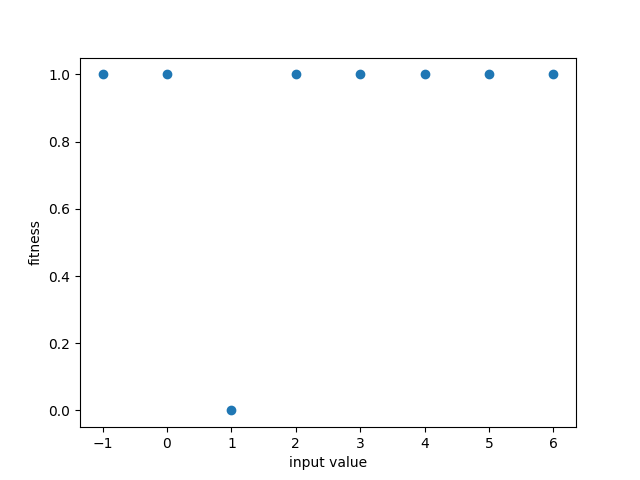
\includegraphics[width=1\textwidth]{figures/plot_no_guidance}
		\end{figure}
		
	\end{columns}	

\end{frame}

\begin{frame}
	\frametitle{Information Content}
	
	\begin{itemize}
		\item \cite{Vassilev.2000}
		\item how many information is needed to construct $S$
	\end{itemize}
	
\end{frame}